\section{Simple Carrier Sensing}
\label{sec:simple}

Simple Carrier Sensing tries to avoid collisions on the channel using a p-persistent approach.
When a station wants to transmit, it checks if the channel is free or occupied.
In the first case, it transmits immediately.
In the second case, it re-schedules the transmission with persistence $p$. $p$ is a probability that defines if the transmission is scheduled immediately after the channel becomes free or postponed of an exponential random time with average $T_r = 10T_t$, where $T_t$ is the time needed to transmit the maximum size packet.

We assume that the scheduled transmissions are cancelled if some packets arrive in the meanwhile.
After the new packet is received and processed, the postponed packet can be eventually transmitted: a new random variable is used to decide whether the packet should be transmitted immediately of postponed again.

\begin{figure}[ht]
	\centering
	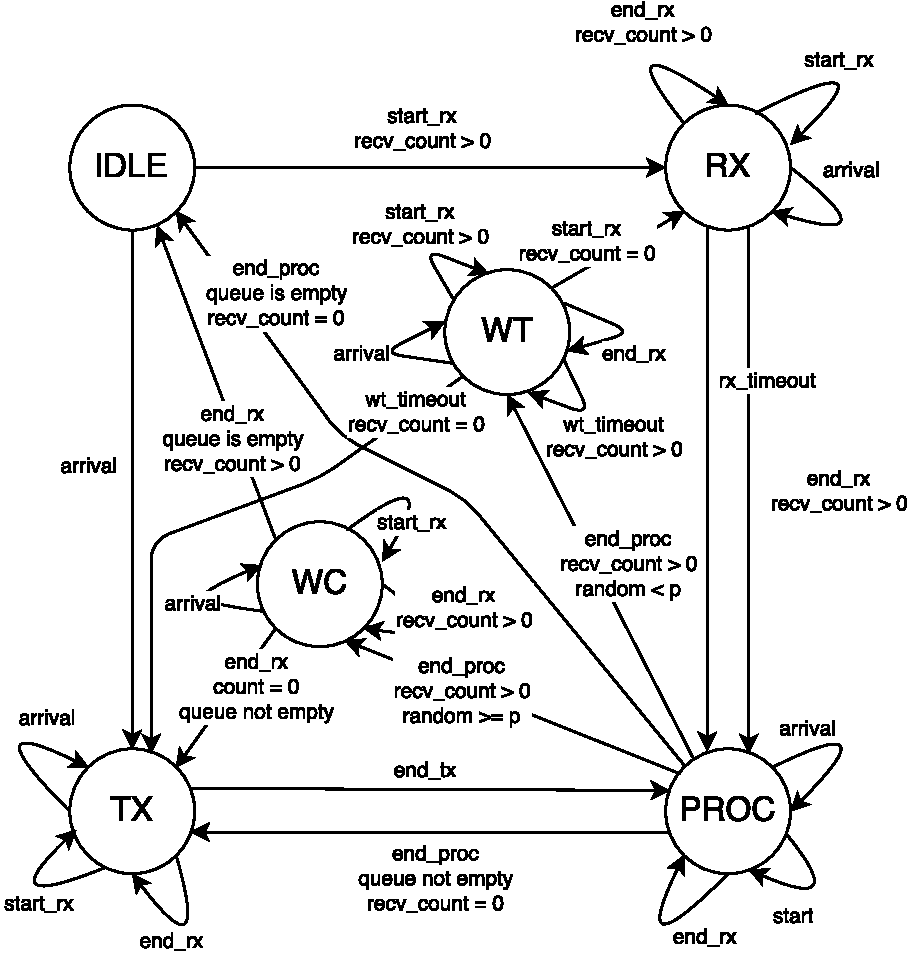
\includegraphics[width=\columnwidth]{figures/states/simple}
	\caption{State machine for a single station for Simple Carrier Sensing.}
	\label{fig:simple_cs_states}
\end{figure}

\cref{fig:trivial_cs_states} shows the state machine diagram for the Simple Carrier Sensing.
The event \textbf{wt\_timeout} indicates the scheduled transmission of a packet.
The new state \textbf{WT} (WAITING\_TO\_TRANSMIT) indicate that the station is idle but waiting to transmit a rescheduled packet.
